
%\setlength{\marginparwidth}{3cm}

\newpage

\section{Inngangur}

Við lifum í heimi sem er umlukinn ýmiskonar tækni. Við notum tækni í flestu sem við tökum okkur fyrir hendur á hverjum degi. Þegar við vöknum þá er það vekjaraklukka sem vekur okkur flest. Við notum ristavélar, notum ísskápa, notum farsima, keyrum bíla og jafnvel notum tækni til að bjarga lífi okkar í formi gangráða og svo framvegis. Mestöll þessi tækni hefur það sameiginlegt að það sem gefur tæknini hæfni til að virka sem skildi er rafmagn.
\\ \\
Fyrir hinn almenna notanda þá getur tæki sem keyrir á rafmagni verið dularfullt og flókið. Ef tekinn er farsimi eða fartölva inn í djúpustu frumskóga heims til frumstæðra þjóðflokka þá getur tæknin sem keyrir tækin virðst sem galdrar eða kraftaverk.
\\ \\
Bók þessari er ætluð þann tilgangur að gefa hinum almenna framhaldsskólanema innsýn inn í hvað rafmagn er, rafmagn virkar og hvernig rafmagn getur verið nýtt til að veita okkur hið tæknivædda umhverfi sem við lifum í.


\section{Hvað er rafmagn?}
Til að svara því hvað rafmagn er þá þurfum við að kíkja i heim atómana. Atom eru byggingarblokkir efnis, semsagt það eru atom í öllu efni hvort sem það er gull, sandur eða loftið sem við öndum að okkur. Þegar atom koma saman þá mynda þau efni og geta þá á einfaldann hátt talist byggingakubbar alls heimsins. Svipað og lego þegar það er samsett myndar kastala, bíla o.s.frv. þá mynda atóm þegar þau eru samsett allt það efni sem við vitum um. 
\\ \\ 
\marginpar{ \hspace{0pt} Rafeind geymir örlitla rafhleðslu.}
Kjarni atóma getur ýmist verið hlaðinn eða óhlaðinn rafeindum. Við réttar aðstæður þá er hægt að láta atom gefa frá sér, eða taka við rafeindum þegar óhlaðin atóm eru sett við hlið hlaðinna. Þegar þetta gerist þá kemst ákveðin hreyfing á rafeindirnar og það myndar, þegar milljónir rafeinda hreyfast í einu, það sem við köllum rafstraum í dag. Mynd 1 sýnir mynd af þessu ferli. Þetta er mjög einfölduð mynd en flestar efnafræði eða eðlisfræðibækur geta gefið betri innsýn inn í þetta ferli, þó er þessi útskýring nægjanleg fyrir það efni hér er fjallað um. 

\begin{figure}
\center
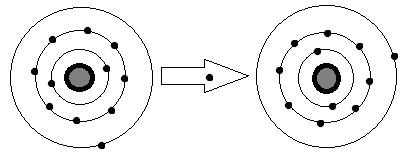
\includegraphics[bb=0 0 408 158]{fig_electrons.jpg}
\caption{Hreyfing rafeinda milli atóma.}
\end{figure}

\section{Grunn einingar rafmagns.}

Rafmagn er hugtak sem í raun er búið til úr þremur grunn einingum, viðámi, straum og spennu. Við getum ýmindað okkur þessi þrjú hugtök í sambandi við rör fyllt af vatni sem flæðir í gegn. Viðnámið taknar það þegar rörið þrengist og gerir vatninu erfiðara um vik að flæða. Straumurinn er magnið af vatni sem flæðir á hverjum stað í rörinu fyrir sig. Spennan er þá þrýstingurinn bakvið vatnið sem lætur það flæða. Nú getum við heimfært þessa líkingu yfir á rafrásir þar sem straumurinn af vatni er straumur af rafeindum, spennan er þrýstingurinn bakvið rafeindirnar myndaðar af rafeindaflæði inn á rasina og viðnám breytir flæði rafeinda, og þar með breytir straumflæði rásarinnar.

\begin{itemize}
\item Spenna er táknuð með stafnum V sem stendur fyrir "Volt". Við höfum öll séð merkingu á batteríum út í verslunum þar sem stendur 9V, 5V o.s.frv. Einnig eru merkingar með spennu gefnar á spennugjöfum við fartölvur, gsm síma og annarskonar tæki sem hlaða rafmagni inn á rafmagnstæki. Volt er skilgreint sem vinnan sem þarf að vera framkvæmd til að flytja rafhleðslu eitt coulomb á milli tveggja punkta. 1 coulomb er skilgreint sem 6.241*10\textsuperscript{18} rafeindir. Ef vinnan er jöfn einu joule þá er spennan á milli þeirra eitt volt. Þessi eining, volt, er einfaldlega hugsuð sem "þrýstingurinn" sem nauðsynlegur er til að færa nægann straum yfir á viðkomandi tæki. 

\item Straumur er táknaður með stafnum I, en er skrifað sem einingin "Ampere". Þetta gefur til kynna að ákveðið magn rafeinda hafi flætt framhjá tilteknum punkt á rafrás á ákveðnu timabili. Eitt Ampere er eitt coulomb á sekúndu. Raftæki geta dregið að sér straum, eða fengið straum þrýst inn á sig með spennu, en straumur getur ekki undir eðlilegum kringumstæðum flætt sjálfstætt.

\item Viðnám er táknað með stafnum R, en er skrifað með gríska stafnum $\Omega$ sem stendur fyrir "Ohm". Viðnám er oft sett inn á rafrásir til að breyta spennu og/eða straum.
\end{itemize}

\section{Ohm lögmálið.}
Eitt mikilvægasta lögmál rafmagnsfræðinnar er kalla "Ohm lögmálið". Þetta er sett upp sem stærðfræðiformúla:
\begin{equation}
V=IR
\end{equation} eða \\ 
\begin{center} Spenna = Straumur * Viðnám \end{center}
Þessi jafna lýsir samhengi milli þessara þriggja þátta sama hlutarins (Rafmagns). En þegar einni stærð er breytt þá breytast hinar stærðirnar um leið.
Með einfaldri algebru þá er hægt að sjá samhengi annara þátta jöfnunar. \\ \\
Fyrir straum:
\begin{equation}
I=\frac{V}{R}
\end{equation}
Fyrir viðnám:
\begin{equation}
R=\frac{V}{I}
\end{equation}
Með því að beita þessum formúlum þá er hægt að leysa stórann hluta allra vandamála sem einstaklingur er líklegur til að lenda á. \\ \\

\begin{enumerate}
\item Viðnáms dæmi.
	\begin{enumerate}
	\item Ef rás vinnur á 5V spennu og 3A straum. Hvað er viðnámið stórt? \\
		\begin{equation}
			\begin{split}
			V&=IR \\
			5V&=3A*R \\
			R&=\frac{5V}{3A}\\
			R&=1.66\Omega
			\end{split}
		\end{equation}
		Semsagt, samkvæmt lögmáli ohm, þá er stærð viðnámsins 1.6$\Omega$. Takið eftir að skref þrjú útreikningsins passar við
		eina útgáfu Ohm lögmálsins hér að ofan.
	\item Ef rás vinnur á 10V spennu og 5mA straum. Hvað er viðnámið stórt?
		\begin{equation}
			\begin{split}
				V&=IR \\
				10V&=0.01A*R \\
				R&=\frac{10V}{0.01A} \\
				R&=1000\Omega
			\end{split}
		\end{equation}
		Takið eftir að þúsund $\Omega$ er oft skrifað sem 1k$\Omega$. Þetta er venja innan rafmagnsfræðinnar, ásamt því að eitt mA er eitt milli ampere, eða 0.001 Ampere.
	\end{enumerate}
\item Straum dæmi.
	\begin{enumerate}
	\item Ef rás vinnur á 5V spennu, og hún fer gegnum 1k$\Omega$ viðnám. Hver er þá stærð straums rásarinnar?
		\begin{equation}
			\begin{split}
			V&=IR \\
			5V&=I*1k\Omega \\
			I&=\frac{5V}{1k\Omega} \\
			I&=0.005A \\
			&=5mA
			\end{split}
		\end{equation}
		Takið eftir hvernig breytt er milli k og þúsund, einnig þá hvernig farið er milli A og mA.
	\end{enumerate}
\item Spennu dæmi.
	\begin{enumerate}
		\item Ef rás hef 2.4k$\Omega$ viðnám, og straum sem fer gegnum það sem er 3mA. Hver er þá stærð spennunnar?
		\begin{equation}
			\begin{split}
			V&=IR \\
			V&=2.4k\Omega*3mA \\
			&=2400\Omega*0.003A \\
			V&=72V
			\end{split}
		\end{equation}
	\end{enumerate}
\end{enumerate}

\section{Aðrar rafeiningar.}
\subsection{Þéttar}
þéttar eru ein grunneininga rafmagnsfræðinnar í íhlutum talið. Viðnám og þéttar eru nægir íhlutir til að framkvæma ýmsar
aðgerðir með rafrásum. Hægt er að horfa á þétti sem hálfgert forðabúr. Þegar auka rafmagn er til staðar þá dregur þéttirinn
það í sig, auk þess sem það jafnar út ýmsar ójöfnur eins og þegar það kemur stutt tímabil þar sem rafmagn vantar, þá getur þéttir
veitt rafmagni úr forðabúrinu til að jafna út þessa ójöfnu svo tækið virki sem skildi. Einingin sem notuð er til að gefa til kynna
hleðslu þétta heitir ''Farad'' eftir englendingnum Michael Faraday. Eins farad þéttir getur hlaðið inn á sig ramagni sem nemur einu coloumb á hvert volt (1C/V) 
eða eina amper sekúndu á volt (1As/V).
\begin{figure}[htb]
	\center
		\includegraphics[bb=0 0 252 262,scale=0.3]{capnres.png}
		\caption{Tákn fyrir þétta (vinstri) og viðnám (hægri).}
\end{figure}

\subsection{Spólur.}
Spólur eru íhlutir í rafrásum sem hafa tvo eiginleika. Þær búa til segulsvið ásamt því að ''hægja'' á straum. Fyrri eiginleikinn nýtist við það að útbúa 
segulmagn og loftnet. Seinni eiginleikinn hefur aðal tilgang í riðstraumsrásum (AC) þar sem spólur nýtast til að breyta lögun rafmerkja. Eining fyrir styrk
spóla er ''Henry''.
\begin{figure}[htb]
	\center
		\includegraphics[bb=0 0 269 130,scale=0.3]{./pictures/inductor.png}
		\caption{Tákn fyrir spólu.}
\end{figure}

\section{Rað og hliðtengingar.}
Við höfum þegar séð hvernig reikna á straum, spennu og viðnám við einföldustu aðstæður. En nú ætlum við að skoða hvernig við reiknum þessa hluti í flóknari
rafrásum.
\begin{figure}[htb]
	\center
		\includegraphics[bb=0 0 873 552,scale=0.3]{./pictures/demo_circ_serpar.png}
		\caption{Einföld rafrás með hlið og raðtengdum íhlutum.}
\end{figure}
Þegar íhlutir eins og viðnám og þéttar eru settir í rásir í rað, eða hliðtengingum þá breytast eiginleikar rásarinnar samkvæmt því. 

\subsection{Viðnám.}
\begin{figure}[htb]
	\center
		\includegraphics[bb=0 0 761 309,scale=0.3]{./pictures/res_parser.png}
		\caption{(a)Hliðtend viðnám. (b)Raðtengd viðnám.}
		\label{fig:res_parser}
\end{figure}
Þegar hlutir gerast! Sjá mynd ~\ref{fig:res_parser}.

\subsection{Þéttar.}
\begin{figure}[htb]
	\center
		\includegraphics[bb=0 0 1056 370,scale=0.3]{./pictures/cap_parser.png}
		\caption{(a)Hliðtendir þéttar. (b)Raðtengdir þéttar.}
		\label{fig:cap_parser}
\end{figure}
Þá gerast hlutir! Sjá mynd ~\ref{fig:cap_parser}.
